\section{Method}

To solve the problem of anomaly detection and image classification, a machine learning pipeline has been developed. The pipeline consists of a anomaly detection procedure that use an autoencoder to reconstruct an input image, calculate the reconstruction error and make a decision based on the error. Images that the anomaly detection procedure considers as anomalies are then passed to a CNN to classify the anomaly. The pipeline is visualized in figure \ref{fig:ml_pipeline}.
\begin{figure}[H]
    \centering
    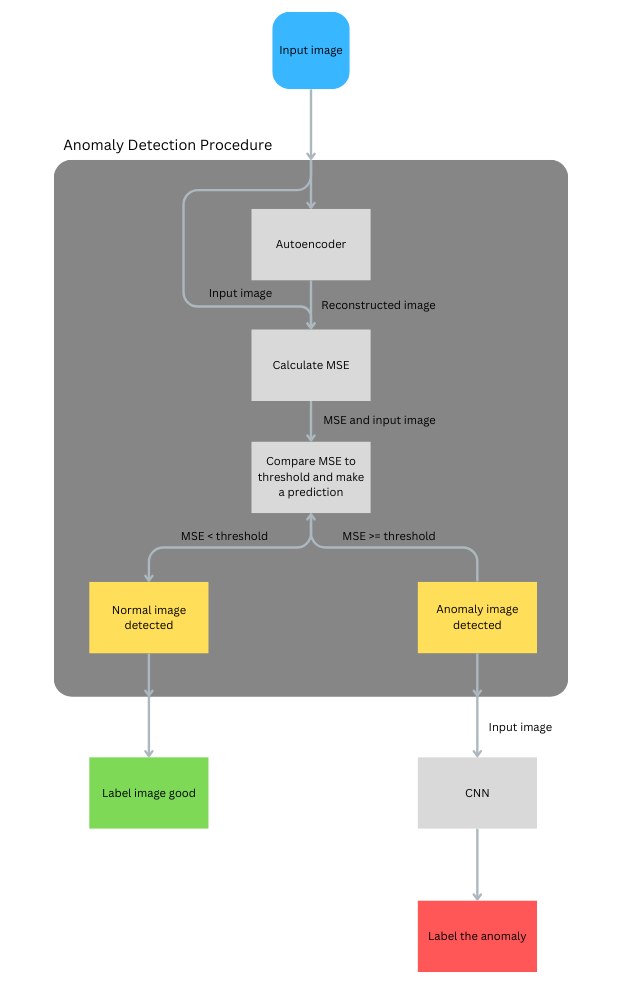
\includegraphics[scale=0.6]{src/images/machine_learning_pipeline.png}
    \caption{Machine learning pipeline visualized}
    \label{fig:ml_pipeline}
\end{figure}

\subsection{Autoencoder}

\subsection{Anomaly detection procedure}

\subsection{CNN}